%Implementierung_vollmatrize
%\subsubsection{Multiplikation von Matrix mit Vektor in CUDA Implementierung}

%Beim Wissenschaftlichen Rechen trifft man häufig die Multiplikation von Matritze mit Vektor. In CUDA Implementierung wird die Oparation als unterschiedliche Vektor-Multiplicationen zerlegt.Mit änlichem Methode werden auch Matizen mit Vektoren multipliziert. Im folgendem Bild Abb.\ref{MatrixVektor}.zeigt, dass jede zerlegte Vektor von $A$ mit Vektor $b$ in einem Block multipliziert wird.

\subsubsection{Matrix-Vektorprodukt}

Die CUDA-Implementierung zerlegt die Matrix-Vektormultiplikation in einzelne
Verktorprodukte.
Abb.\ref{MatrixVektor} zeigt wie die Teilvektoren von $ \bf A$ mit dem Vektor $ \bf b$
innerhalb eines Blockes multipliziert werden.


\begin{figure}[htbp]
\centering
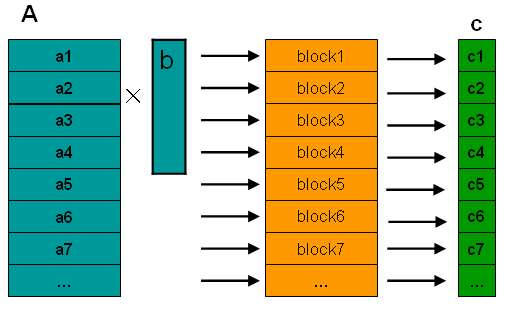
\includegraphics[width=2.8in]{../xby/pic//MatrixVektor}
\caption{ \label{MatrixVektor} Matrix-Vektorprodukt: Multiplikand $\bf A$, Multiplikator $ \bf b$, Produkt $\bf c$ }

\end{figure}